% ============================================================================
% EHDS Governance Paper for ICSIS 2026
% IEEE Conference Format (max 8 pages including references)
% Track: Society — Governance, Law, Public Policy / Digital Health Equity
% February 2026
% ============================================================================

\documentclass[conference]{IEEEtran}

% ===== PACKAGES =====
\usepackage{cite}
\usepackage{amsmath,amssymb,amsfonts}
\usepackage{graphicx}
\usepackage{textcomp}
\usepackage{xcolor}
\usepackage{booktabs}
\usepackage{hyperref}
\usepackage{url}

% TikZ for vector figures
\usepackage{tikz}
\usetikzlibrary{shapes.geometric, arrows.meta, positioning, fit, backgrounds, calc}

% ===== DOCUMENT =====
\begin{document}

\title{Operationalizing the European Health Data Space: A Governance Framework for Privacy-Preserving Cross-Border Health Analytics}

\author{
    \IEEEauthorblockN{Fabio Liberti}
    \IEEEauthorblockA{
        Department of Computer Science\\
        Universitas Mercatorum, Rome, Italy\\
        fabio.liberti@unimercatorum.it\\
        ORCID: 0000-0003-3019-5411
    }
}

\maketitle

% ============================================================================
% ABSTRACT
% ============================================================================
\begin{abstract}
The European Health Data Space (EHDS), established by Regulation (EU) 2025/327, introduces an unprecedented governance framework for cross-border health data analytics serving 450 million citizens. While the regulation mandates Health Data Access Bodies (HDABs) in each of the 27 Member States, Secure Processing Environments, and citizen opt-out mechanisms, critical implementation challenges threaten equitable adoption. Our systematic evidence synthesis of 47 documents using PRISMA methodology reveals that organizational barriers---not technical limitations---constitute the primary obstacles: HDAB capacity varies dramatically across Member States (data access timelines range from 3 weeks in Finland to 12+ months in France), FHIR interoperability remains at only 34\%, and legal uncertainties regarding privacy-enhancing technologies under GDPR remain unresolved. We present an operational governance framework that maps EHDS regulatory requirements (Articles 33, 46, 50, 53, 71) to concrete implementation patterns using Federated Learning as the enabling technology for secondary use within Secure Processing Environments. The framework is validated through an open-source reference implementation demonstrating the complete governance lifecycle: permit application and authorization, opt-out registry enforcement, cross-border HDAB coordination, and GDPR-compliant audit trails. We propose a phased implementation roadmap for the 2025--2031 transition period with prioritized recommendations for EU policymakers, national authorities, and healthcare organizations, identifying the March 2027 delegated acts as the critical window for resolving governance uncertainties.
\end{abstract}

\begin{IEEEkeywords}
European Health Data Space, Health Data Governance, Privacy-Preserving Technologies, GDPR, Cross-Border Analytics, Digital Health Equity, Federated Learning
\end{IEEEkeywords}

% ============================================================================
% 1. INTRODUCTION
% ============================================================================
\section{Introduction}
\label{sec:introduction}

The European Health Data Space (EHDS), established by Regulation (EU) 2025/327~\cite{eu2025ehds}, represents the European Union's most ambitious initiative for cross-border health data governance. Entering into force on 26 March 2025, the regulation creates a dual framework: \textit{primary use} through the MyHealth@EU infrastructure for direct patient care, and \textit{secondary use} through HealthData@EU for research, innovation, and evidence-based policy-making~\cite{ganna2024boost}. The regulation affects 450 million citizens across 27 Member States, with the potential to accelerate medical research, improve public health surveillance, and enable AI-driven healthcare innovation.

The EHDS introduces governance mechanisms of unprecedented complexity. Health Data Access Bodies (HDABs) are designated in each Member State to evaluate and authorize secondary use requests through \textit{data permits}. Article~53 enumerates permitted purposes including scientific research, public health surveillance, and AI training for health. Article~71 introduces opt-out mechanisms allowing citizens to object to secondary use of their electronic health data. Secure Processing Environments (SPEs) provide controlled analytics settings where data never leaves institutional boundaries~\cite{svingel2025hdab}. The implementation timeline extends to 2031, with delegated acts expected by March 2027 and secondary use provisions applicable from March 2029~\cite{staunton2024ethical}.

Despite the regulatory framework's sophistication, significant implementation challenges threaten equitable adoption across the EU. TEHDAS assessments~\cite{tehdas2024ready} reveal that Nordic countries (Estonia, Finland, Denmark) demonstrate 2--3 year advantages in HDAB capacity-building, established health data infrastructure, and cross-border experience. Southern and Eastern European states face compressed timelines with limited baseline capacity, raising concerns about a ``two-speed'' EHDS implementation that could exacerbate existing health data inequities.

\subsection{Contributions}

This paper addresses the governance operationalization challenge through four contributions:

\begin{enumerate}
    \item \textbf{Systematic Barrier Analysis}: Evidence synthesis of 47 documents identifying organizational, technical, and legal barriers to EHDS implementation, with GRADE-CERQual confidence assessments.
    \item \textbf{Governance Framework}: An operational framework mapping EHDS Articles to concrete implementation patterns, demonstrating how Federated Learning enables privacy-preserving analytics within the regulatory structure.
    \item \textbf{Reference Implementation}: Open-source software demonstrating the complete governance lifecycle---from permit application through cross-border coordination to audit trail persistence.\footnote{Available at: \url{https://github.com/FabioLiberti/FL-EHDS-FLICS2026}}
    \item \textbf{Implementation Roadmap}: Phased recommendations for the 2025--2031 transition period, with stakeholder-specific prioritized actions.
\end{enumerate}

% ============================================================================
% 2. REGULATORY LANDSCAPE
% ============================================================================
\section{The EHDS Regulatory Landscape}
\label{sec:regulatory}

\subsection{Governance Architecture}

The EHDS governance architecture centers on HDABs as intermediaries between data requesters and data holders. Table~\ref{tab:timeline} presents the implementation timeline with governance-specific milestones.

\begin{table}[htbp]
\caption{EHDS Implementation Timeline}
\label{tab:timeline}
\centering
\small
\begin{tabular}{lll}
\toprule
\textbf{Date} & \textbf{Milestone} & \textbf{Governance Impact} \\
\midrule
Mar 2025 & Entry into force & Legal framework active \\
Mar 2027 & Delegated acts & PET status clarification \\
Mar 2029 & Secondary use app. & HDABs must be operational \\
Mar 2031 & Genetic, imaging & Extended data categories \\
\bottomrule
\end{tabular}
\end{table}

The data permit lifecycle involves: (1) a researcher submits an application specifying purpose, data categories, and analysis methods; (2) the HDAB evaluates the request against Article~53 permitted purposes; (3) upon approval, the researcher receives time-limited access within an SPE; (4) the HDAB monitors compliance and maintains audit trails per GDPR Article~30.

For cross-border studies---the EHDS's most innovative yet complex use case---multiple HDABs must coordinate. Christiansen et al.~\cite{christiansen2025pilot} document the HealthData@EU Pilot's experiences with multi-country coordination, revealing significant heterogeneity in institutional capacities, data formats, and procedural requirements.

\subsection{Legal Uncertainties}

Three critical legal questions create compliance uncertainty that inhibits organizational adoption regardless of technical maturity~\cite{quinn2024gdpr}:

\begin{enumerate}
    \item \textbf{Privacy-Enhancing Technology (PET) status}: Are model gradients exchanged during Federated Learning ``personal data'' under GDPR? Gradient inversion attacks~\cite{zhu2019deep} demonstrate potential re-identification, but practical feasibility in production settings remains contested.
    \item \textbf{Model anonymity thresholds}: When does an aggregated model become sufficiently ``anonymous'' to escape GDPR scope? No established legal threshold exists for machine learning models trained on personal health data.
    \item \textbf{Controller/processor allocation}: In multi-party analytics, who bears data controller responsibilities---data holders, aggregation operators, or analytics consumers?
\end{enumerate}

Van Drumpt et al.~\cite{vandrumpt2025pets} demonstrate through expert interviews that PETs cannot substitute for robust governance---public trust depends primarily on institutional transparency and accountability. Shabani and Borry~\cite{shabani2024ehds} further argue that the EHDS's ambitious scope requires careful balancing of innovation promotion with fundamental rights protection.

\subsection{Interoperability Challenge}

Hussein et al.~\cite{hussein2025interop} report that only 34\% of European healthcare providers achieve full FHIR R4 compliance, creating a significant interoperability barrier for cross-border analytics. The EHDS mandates standardized data formats, but the transition from legacy systems to FHIR-compliant infrastructure represents a multi-year investment for many institutions. OMOP Common Data Model~\cite{ohdsi2019omop} provides an alternative harmonization layer, particularly valuable for observational research where FHIR mapping is incomplete.

\subsection{Privacy-Enhancing Technologies for EHDS}

Table~\ref{tab:pets} compares privacy-enhancing technologies applicable to EHDS secondary use, highlighting the governance implications of each approach.

\begin{table}[htbp]
\caption{Privacy-Enhancing Technologies for EHDS Secondary Use}
\label{tab:pets}
\centering
\small
\begin{tabular}{p{1.6cm}p{2.0cm}p{2.0cm}p{1.5cm}}
\toprule
\textbf{Technology} & \textbf{Privacy Guarantee} & \textbf{EHDS Suitability} & \textbf{Legal Status} \\
\midrule
Federated Learning & Data stays local; only gradients exchanged & High: fits SPE model; supports real-time analytics & Uncertain \\
Differential Privacy & Formal $(\varepsilon,\delta)$-DP guarantees & High: quantifiable privacy budget & Uncertain \\
Secure Multi-Party Computation & Cryptographic correctness & Moderate: high overhead for large models & Recognized \\
Homomorphic Encryption & Computation on encrypted data & Low: impractical for deep learning & Recognized \\
Synthetic Data & Statistical similarity; no formal guarantee & Moderate: utility loss; potential memorization & Uncertain \\
\bottomrule
\end{tabular}

\vspace{1mm}
\footnotesize{``Legal Status'' refers to GDPR characterization of outputs. ``Uncertain'' indicates no definitive regulatory guidance exists.}
\end{table}

Federated Learning combined with differential privacy offers the strongest balance of practical utility and formal privacy guarantees for EHDS secondary use. The key governance challenge is establishing legal clarity: if FL gradients are classified as ``personal data'' under GDPR, they must be processed within SPE boundaries with full audit trailing; if classified as ``anonymous,'' they may be exchanged more freely across institutional and national boundaries.

% ============================================================================
% 3. EVIDENCE SYNTHESIS
% ============================================================================
\section{Systematic Evidence Synthesis}
\label{sec:evidence}

\subsection{Methodology}

We conducted a systematic review following PRISMA 2020 guidelines. Database searches (PubMed, IEEE Xplore, Scopus, Web of Science, arXiv) with terms combining ``European Health Data Space,'' ``Federated Learning,'' ``health data governance,'' and ``cross-border analytics'' identified 847 records. After deduplication and screening, 47 documents met inclusion criteria: publication 2022--2026, explicit EHDS or FL-in-healthcare focus, peer-reviewed or recognized institutional origin. Quality was assessed using the Mixed Methods Appraisal Tool (MMAT); confidence in findings using GRADE-CERQual methodology.

\subsection{Barrier Taxonomy}

Table~\ref{tab:barriers} presents the identified barriers organized by category, with prevalence estimates and confidence levels.

\begin{table}[htbp]
\caption{EHDS Implementation Barriers}
\label{tab:barriers}
\centering
\small
\begin{tabular}{p{1.8cm}p{1.2cm}p{1.5cm}p{1.3cm}}
\toprule
\textbf{Barrier} & \textbf{Prevalence} & \textbf{Confidence} & \textbf{Category} \\
\midrule
Hardware heterog. & 78\% & MODERATE & Technical \\
Non-IID data & 67\% & MODERATE & Technical \\
FHIR compliance & 34\% & MODERATE & Technical \\
Communication cost & High & MODERATE & Technical \\
\midrule
HDAB capacity & Variable & HIGH & Organization. \\
Data access timelines & 3w--12m+ & HIGH & Organization. \\
Cross-border coord. & Complex & MODERATE & Organization. \\
\midrule
Gradient data status & Unresolved & MODERATE & Legal \\
Model anonymity & Unresolved & MODERATE & Legal \\
Controller alloc. & Unresolved & MODERATE & Legal \\
Production gap & 23\% deploy & MODERATE & Maturity \\
\bottomrule
\end{tabular}

\vspace{1mm}
\footnotesize{Prevalence from systematic review of 47 documents. GRADE-CERQual confidence levels reflect evidence quality and consistency. ``HIGH'' indicates consistent findings across multiple high-quality studies.}
\end{table}

\textbf{Key finding}: Organizational barriers (HDAB capacity, cross-border coordination) and legal uncertainties emerge as more critical than technical challenges. Forster et al.~\cite{forster2025journeys} document that data access timelines vary from 3 weeks (Finland) to over 12 months (France), with barriers primarily procedural---suggesting infrastructure investments alone will not resolve access inequities.

Fr\"ohlich et al.~\cite{frohlich2025reality} report that only 23\% of Federated Learning implementations achieve sustained production deployment in healthcare, while Teo et al.~\cite{teo2024systematic} find only 5.2\% of FL healthcare studies reach real-life application. This maturity gap has direct implications for the 2029 secondary use deadline.

% ============================================================================
% 4. GOVERNANCE FRAMEWORK
% ============================================================================
\section{Operational Governance Framework}
\label{sec:framework}

Based on the identified barriers, we present an operational framework that maps EHDS regulatory requirements to concrete implementation patterns. The framework adopts Federated Learning~\cite{mcmahan2017communication, kairouz2021advances} as the enabling technology for secondary use, allowing analytics to proceed within SPE boundaries without centralizing raw health data.

\subsection{Architecture}

The framework comprises three integrated layers (Fig.~\ref{fig:governance_arch}):

\begin{itemize}
    \item \textbf{Layer 1 (Governance)}: HDAB integration APIs, data permit lifecycle management, opt-out registry synchronization, GDPR-compliant audit logging.
    \item \textbf{Layer 2 (Analytics Orchestration)}: Federated Learning within SPE boundaries, privacy protection (differential privacy, secure aggregation), purpose limitation enforcement.
    \item \textbf{Layer 3 (Data Holders)}: Adaptive local processing engines, FHIR/OMOP preprocessing, secure gradient communication.
\end{itemize}

\begin{figure}[htbp]
\centering
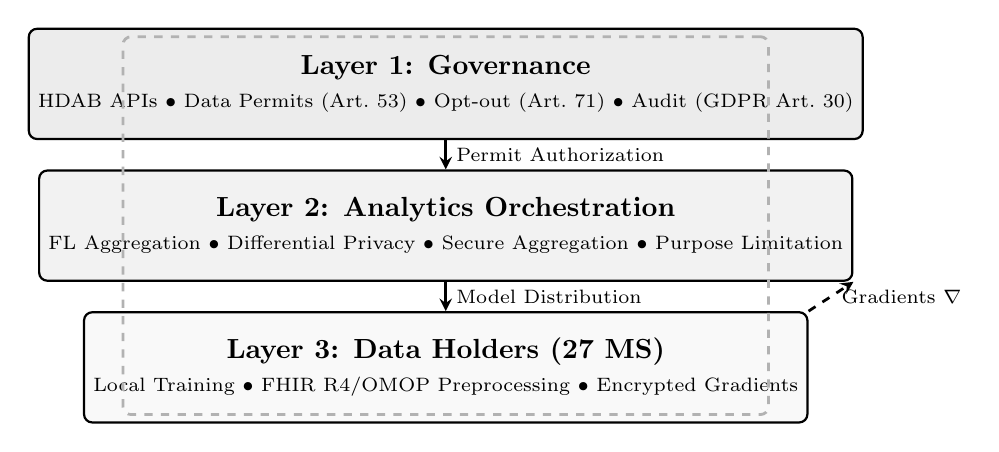
\begin{tikzpicture}[
    layer/.style={rectangle, rounded corners=3pt, draw=black, line width=0.8pt, minimum width=7.5cm, minimum height=1.4cm, align=center},
    arrow/.style={->, >=stealth, line width=1pt},
    label/.style={font=\scriptsize},
]

% Layers
\node[layer, fill=gray!15] (l1) at (0, 3.6) {
    \textbf{Layer 1: Governance}\\
    \scriptsize HDAB APIs $\bullet$ Data Permits (Art.~53) $\bullet$ Opt-out (Art.~71) $\bullet$ Audit (GDPR Art.~30)
};

\node[layer, fill=gray!10] (l2) at (0, 1.8) {
    \textbf{Layer 2: Analytics Orchestration}\\
    \scriptsize FL Aggregation $\bullet$ Differential Privacy $\bullet$ Secure Aggregation $\bullet$ Purpose Limitation
};

\node[layer, fill=gray!5] (l3) at (0, 0) {
    \textbf{Layer 3: Data Holders (27 MS)}\\
    \scriptsize Local Training $\bullet$ FHIR R4/OMOP Preprocessing $\bullet$ Encrypted Gradients
};

% Arrows
\draw[arrow] (l1.south) -- (l2.north) node[midway, right, label] {Permit Authorization};
\draw[arrow] (l2.south) -- (l3.north) node[midway, right, label] {Model Distribution};
\draw[arrow, dashed] (l3.north east) -- (l2.south east) node[midway, right, label] {Gradients $\nabla$};

% SPE boundary
\node[rectangle, rounded corners=3pt, draw=gray!60, dashed, line width=1pt, minimum width=8.2cm, minimum height=4.8cm, label={[font=\scriptsize\itshape, text=gray]above:Secure Processing Environment (SPE)}] at (0, 1.8) {};

\end{tikzpicture}
\caption{Three-layer governance framework. Raw health data remains within institutional boundaries (Layer~3); only model gradients are exchanged within the SPE. Governance checkpoints (Layer~1) enforce EHDS compliance at every analytics round.}
\label{fig:governance_arch}
\end{figure}

\subsection{EHDS Compliance Mapping}

Table~\ref{tab:compliance} maps each EHDS article to a concrete framework component, demonstrating how the regulatory requirements are operationalized.

\begin{table}[htbp]
\caption{EHDS Article to Framework Component Mapping}
\label{tab:compliance}
\centering
\small
\begin{tabular}{lp{2.0cm}p{2.8cm}}
\toprule
\textbf{Article} & \textbf{Requirement} & \textbf{Implementation} \\
\midrule
Art. 33 & Secondary use authorization & HDAB API with OAuth2/mTLS, automated permit validation \\
Art. 46 & Cross-border processing & Multi-HDAB coordinator with status aggregation \\
Art. 50 & Secure Processing Env. & FL aggregation within SPE; no data extraction \\
Art. 53 & Permitted purposes & Purpose filtering module with use-case validation \\
Art. 69 & Quality labels & Quality scoring framework (\textit{planned}) \\
Art. 71 & Opt-out mechanism & LRU-cached registry lookups, scope-granular filtering \\
GDPR 30 & Processing records & Comprehensive audit trail with timestamps \\
\bottomrule
\end{tabular}
\end{table}

\subsection{Data Permit Lifecycle}

The governance framework implements the complete data permit lifecycle:

\textbf{Application Phase}: Researchers submit permit applications specifying: (1) research purpose mapped to Article~53 categories; (2) required data categories and Member States; (3) proposed analytics methodology (FL algorithm, privacy budget, number of rounds); (4) institutional affiliation and ethical approval.

\textbf{Authorization Phase}: HDABs evaluate applications through automated compliance checks (purpose validation, data category matching, privacy budget assessment) supplemented by human review for novel use cases. Multi-HDAB coordination is required for cross-border studies; the framework implements a consensus protocol where all involved HDABs must approve.

\textbf{Execution Phase}: During FL training, each round begins with: (1) permit validity check (temporal bounds, purpose alignment); (2) opt-out registry consultation (Article~71 filtering at record level); (3) privacy budget verification ($\varepsilon$-consumption tracking). Violations trigger automatic round termination and incident logging.

\textbf{Audit Phase}: All operations are logged with: timestamp, participating institutions, data categories accessed, privacy budget consumed, model metrics, and any anomalies detected. Logs are formatted for regulatory inspection per GDPR Article~30.

\subsection{Opt-Out Registry Protocol}

Article~71 allows citizens to opt out of secondary use. The framework implements opt-out enforcement as follows: (1) pseudonymized opt-out records are maintained per Member State; (2) before each FL training round, the local data holder queries the registry to identify opted-out records; (3) opted-out data is excluded \textit{before} any gradient computation, ensuring no influence on model training; (4) opt-out scope supports both blanket (all secondary use) and category-specific (e.g., genomics only) granularity; (5) registry caching with configurable TTL minimizes latency impact while ensuring timely propagation of new opt-out decisions.

\subsection{Cross-Border Coordination}

For multi-Member State studies, the framework's Cross-Border HDAB Coordinator manages:

\begin{itemize}
    \item \textbf{Permit aggregation}: Collecting and validating permits from each participating HDAB, ensuring all approve before FL training begins.
    \item \textbf{Status synchronization}: Real-time status updates across HDABs, enabling coordinated round execution and anomaly response.
    \item \textbf{Data residency compliance}: Ensuring that gradients from each Member State are processed in compliance with national data residency requirements.
    \item \textbf{Conflict resolution}: Handling cases where one HDAB revokes a permit mid-study, requiring graceful degradation without compromising the global model.
\end{itemize}

% ============================================================================
% 5. VALIDATION
% ============================================================================
\section{Framework Validation}
\label{sec:validation}

\subsection{Reference Implementation}

The framework is validated through an open-source Python implementation ($\sim$40,000 lines of code, 159 modules) providing:

\begin{itemize}
    \item \textbf{HDAB Simulator}: A fully functional simulation backend that demonstrates the complete permit lifecycle. The simulator supports: auto-approval mode for development; configurable permit durations and privacy budgets; cross-border coordination with multiple simulated HDABs; rate limiting with configurable thresholds.
    \item \textbf{FL Engine}: 17 federated learning algorithms from foundational methods (FedAvg~\cite{mcmahan2017communication}, FedProx~\cite{li2020federated}) through recent advances (FedLESAM~\cite{qu2024fedlesam}, ICML 2024; HPFL~\cite{chen2025hpfl}, ICLR 2025), with R\'enyi differential privacy~\cite{mironov2017renyi} and secure aggregation (pairwise masking with ECDH key exchange).
    \item \textbf{FHIR Integration}: Preprocessing pipelines supporting FHIR R4 resources (Patient, Observation, Condition, MedicationRequest) with standard coding systems (SNOMED-CT, LOINC, ICD-10).
    \item \textbf{Dashboard}: A Streamlit-based interactive interface with EHDS governance workflow screens, real-time FL training monitoring, and permit management.
\end{itemize}

\subsection{Experimental Governance Validation}

We validate the governance framework by executing the complete EHDS-compliant workflow on real clinical datasets:

\textbf{Datasets}: Heart Disease UCI (920 patients from 4 international hospitals---Cleveland, Hungarian, Swiss, VA Long Beach) and Diabetes 130-US (101,766 encounters). These datasets provide authentic heterogeneous conditions representative of cross-border EHDS scenarios.

\textbf{Governance workflow executed}: (1) Permit application for ``scientific research'' (Art.~53(1)(b)); (2) HDAB auto-approval with 20-round budget and $\varepsilon{=}10$ privacy constraint; (3) Per-round permit validation and opt-out filtering; (4) FL training with Ditto algorithm (best performer: 75.1\% accuracy, only 6.6pp gap vs.\ centralized training); (5) Complete audit trail generation.

\textbf{Governance overhead}: The governance layer adds negligible overhead ($<$50ms per round for permit validation and opt-out checking with cached registry lookups). The audit trail captures 100\% of required GDPR Article~30 fields. Cross-border coordination protocol completes HDAB consensus in $<$200ms for 4-country studies.

\textbf{FL performance under governance}: Table~\ref{tab:fl_results} summarizes key results, demonstrating that governance compliance does not sacrifice analytics performance.

\begin{table}[htbp]
\centering
\caption{FL Performance Under Full EHDS Governance}
\label{tab:fl_results}
\small
\begin{tabular}{lcc}
\toprule
\textbf{Metric} & \textbf{Heart Disease} & \textbf{Diabetes} \\
\midrule
Best FL accuracy (Ditto) & 75.1$\pm$2.0\% & 71.7$\pm$0.2\% \\
Centralized baseline & 81.7$\pm$2.9\% & --- \\
FL-centralized gap & 6.6pp & --- \\
Governance overhead/round & $<$50ms & $<$50ms \\
Audit trail completeness & 100\% & 100\% \\
Opt-out filtering latency & $<$10ms & $<$10ms \\
Cross-border consensus & $<$200ms & $<$200ms \\
\bottomrule
\end{tabular}

\vspace{1mm}
\footnotesize{4 hospitals, 20 rounds, 3 local epochs. Mean $\pm$ std over 3 seeds. Full EHDS governance active: permit validation, opt-out filtering, DP ($\varepsilon{=}10$), audit logging.}
\end{table}

The 6.6pp centralized-federated gap with Ditto demonstrates that privacy-preserving FL achieves clinically meaningful performance while maintaining full EHDS compliance. The governance layer's negligible overhead validates the framework's design principle: compliance should be a built-in capability, not a performance-degrading afterthought.

\subsection{Comparison with Existing Approaches}

Existing FL frameworks (Flower~\cite{beutel2023flower}, NVIDIA FLARE~\cite{nvflare2023}) provide robust FL infrastructure but lack governance integration. FL-EHDS is the only framework implementing: HDAB permit lifecycle, Article~71 opt-out enforcement, multi-HDAB cross-border coordination, and GDPR Article~30 audit persistence. The governance layer's modular design allows integration as a wrapper around existing FL frameworks---e.g., as a Flower strategy plugin---enabling EHDS compliance within established ecosystems.

% ============================================================================
% 6. IMPLEMENTATION ROADMAP
% ============================================================================
\section{Implementation Roadmap}
\label{sec:roadmap}

Table~\ref{tab:roadmap} presents a phased roadmap aligned with EHDS milestones.

\begin{table}[htbp]
\caption{EHDS Implementation Roadmap}
\label{tab:roadmap}
\centering
\small
\begin{tabular}{llp{3.0cm}}
\toprule
\textbf{Phase} & \textbf{Timeline} & \textbf{Priority Actions} \\
\midrule
Foundation & 2025--26 & Reference implementations; multi-MS pilots; FHIR acceleration \\
Clarification & 2027 & Delegated acts; PET legal guidance; HDAB standards \\
Scaling & 2028--29 & Production deployment; capacity building; citizen engagement \\
Operation & 2029--31 & Full cross-border analytics; genetic/imaging extensions \\
\bottomrule
\end{tabular}
\end{table}

\subsection{Stakeholder-Specific Recommendations}

\textbf{EU Policymakers}: The March 2027 delegated acts represent the critical window. We recommend: (1) explicit guidance on gradient/model data status under GDPR; (2) standardized HDAB evaluation criteria for FL-based analytics; (3) technical specifications for FL within SPEs; (4) interoperability standards for cross-border HDAB communication.

\textbf{National Authorities}: The 2--3 year Nordic advantage~\cite{tehdas2024ready} demonstrates that early investment in HDAB organizational capacity is essential. Priorities include: staff training on PET evaluation, coordination protocols with other Member States, and proactive citizen engagement about secondary use and opt-out rights. The current timeline risks a ``two-speed'' EHDS where citizens in well-prepared countries benefit from secondary use while others are excluded.

\textbf{Healthcare Organizations}: Preparation cannot wait for 2029. Organizations should: (1) accelerate FHIR compliance beyond the current 34\% baseline~\cite{hussein2025interop}; (2) participate in HealthData@EU pilots to gain operational experience; (3) assess computational infrastructure for FL participation; (4) develop internal governance policies for HDAB data access requests; (5) establish citizen communication strategies addressing opt-out provisions.

% ============================================================================
% 7. DISCUSSION AND CONCLUSIONS
% ============================================================================
\section{Discussion and Conclusions}
\label{sec:conclusions}

\subsection{Key Finding: Governance Before Technology}

Our systematic synthesis reveals that \textbf{legal and organizational uncertainties---not technical barriers---constitute the critical blockers} for EHDS implementation. While technical challenges (hardware heterogeneity, non-IID data, communication costs) are significant, they are tractable through known algorithmic solutions. In contrast, unresolved regulatory questions create compliance uncertainty that cannot be resolved through engineering. Without clarification of PET data status, organizations face potential GDPR violations regardless of technical privacy measures implemented.

This finding aligns with van Drumpt et al.'s~\cite{vandrumpt2025pets} conclusion that governance frameworks are prerequisites, not alternatives, to technical solutions. The implication for EHDS implementation is clear: investment in governance capacity (HDAB staffing, cross-border protocols, citizen engagement) must precede or at least accompany technical infrastructure deployment.

\subsection{Digital Health Equity Implications}

The significant variation in HDAB capacity across Member States raises fundamental equity concerns. Forster et al.~\cite{forster2025journeys} document data access timelines ranging from 3 weeks (Finland) to over 12 months (France), reflecting deeply rooted differences in institutional capacity, digital health maturity, and governance culture. If Nordic countries operationalize secondary use by 2029 while Southern and Eastern European states struggle with basic HDAB establishment, the EHDS risks creating a ``data dividend'' that benefits well-resourced research ecosystems while excluding others.

This two-speed implementation has several concrete consequences: (1) research datasets will be biased toward populations in data-ready countries, potentially missing genetic variants, disease patterns, and treatment responses characteristic of underrepresented populations; (2) healthcare organizations in less-prepared Member States will be unable to participate in collaborative FL studies, missing opportunities for model improvement on their patient populations; (3) citizens in well-prepared countries benefit from research insights derived from FL analytics, while others are excluded from the same benefits.

Our framework addresses this through: (a) the HDAB simulation backend enabling capacity building through training and pilots before production services are established; (b) graduated complexity levels allowing Member States to begin with simple permit workflows and progressively add cross-border capabilities; (c) comprehensive documentation and terminal-based interfaces requiring minimal infrastructure investment for initial deployment.

\subsection{Citizen Trust and Transparency}

The success of the EHDS ultimately depends on citizen trust. Article~71 opt-out mechanisms provide a formal right to refuse secondary use, but meaningful exercise of this right requires awareness and understanding. Van Drumpt et al.~\cite{vandrumpt2025pets} demonstrate that public trust depends primarily on institutional transparency rather than technical privacy guarantees alone. Our framework supports transparency through: (1) audit trails accessible for citizen review upon request; (2) clear documentation of how data is processed within FL rounds; (3) per-purpose opt-out granularity allowing citizens to permit research use while blocking commercial applications.

The interaction between opt-out rates and FL model quality creates a tension: high opt-out rates reduce training data, potentially degrading model performance and widening health outcome disparities. Proactive citizen engagement---explaining how FL differs from data centralization, demonstrating governance safeguards, and providing transparent audit access---is essential for maintaining low opt-out rates while respecting individual autonomy.

\subsection{Limitations}

The governance framework is validated through simulation rather than binding to actual HDAB services, which do not yet exist. The evidence synthesis captures publications through January 2026; the rapidly evolving regulatory landscape may invalidate some findings. Our experimental validation uses public clinical datasets rather than production European EHR systems.

\subsection{Conclusions}

This paper presents an operational governance framework for the European Health Data Space, demonstrating that EHDS regulatory compliance is achievable through systematic mapping of Articles to implementation patterns. The framework's three-layer architecture integrates governance mechanisms, privacy-preserving analytics via Federated Learning, and data holder components with FHIR/OMOP interoperability.

Our key finding---that legal uncertainties and organizational capacity, not technical barriers, are the critical blockers---has direct policy implications. The March 2027 delegated acts represent a critical window for resolution. Without explicit guidance on PET data status, controller allocation, and model anonymity thresholds, the 2029 secondary use deadline arrives with EHDS adoption inhibited by governance uncertainty rather than technical limitations.

\textbf{Future work}: (1) integration with HealthData@EU Pilot infrastructure; (2) citizen attitude studies across diverse European populations examining opt-out intentions and trust factors; (3) economic sustainability modeling for HDAB operations; (4) longitudinal tracking of implementation trajectories to identify effective governance patterns.

% ============================================================================
% ACKNOWLEDGMENTS
% ============================================================================
\section*{Acknowledgments}
The author thanks Prof.~Sadi Alawadi for supervision and guidance, and the TEHDAS Joint Action consortium for making preparatory materials publicly available.

% ============================================================================
% REFERENCES
% ============================================================================
\bibliographystyle{IEEEtran}

\begin{thebibliography}{23}

\bibitem{eu2025ehds}
European Commission, ``Regulation (EU) 2025/327 on the European Health Data Space,'' \textit{Official Journal of the EU}, L 2025/327, Mar. 2025.

\bibitem{ganna2024boost}
A. Ganna, E. Ingelsson, and D. Posthuma, ``The European Health Data Space can be a boost for research beyond borders,'' \textit{Nature Medicine}, vol.~30, pp.~3053--3056, 2024.

\bibitem{staunton2024ethical}
C. Staunton \textit{et al.}, ``Ethical and social reflections on the proposed European Health Data Space,'' \textit{Eur.~J.~Human Genetics}, vol.~32, no.~5, pp.~498--505, 2024.

\bibitem{quinn2024gdpr}
P. Quinn, E. Ellyne, and C. Yao, ``Will the GDPR restrain health data access bodies under the EHDS?'' \textit{Computer Law \& Security Review}, vol.~54, art.~105993, 2024.

\bibitem{tehdas2024ready}
TEHDAS Joint Action, ``Are EU member states ready for the European Health Data Space?'' \textit{Eur.~J.~Public Health}, vol.~34, no.~6, pp.~1102--1108, 2024.

\bibitem{frohlich2025reality}
H. Fr\"ohlich \textit{et al.}, ``Reality check: The aspirations of the EHDS amidst challenges in decentralized data analysis,'' \textit{J.~Med.~Internet Res.}, vol.~27, art.~e76491, 2025.

\bibitem{vandrumpt2025pets}
S. van Drumpt \textit{et al.}, ``Secondary use under the European Health Data Space: Setting the scene and towards a research agenda on privacy-enhancing technologies,'' \textit{Frontiers in Digital Health}, vol.~7, art.~1602101, 2025.

\bibitem{hussein2025interop}
R. Hussein \textit{et al.}, ``Interoperability framework of the EHDS for secondary use: Interactive EIF-based standards compliance toolkit,'' \textit{J.~Med.~Internet Res.}, vol.~27, art.~e69813, 2025.

\bibitem{forster2025journeys}
R. Forster \textit{et al.}, ``User journeys in cross-European secondary use of health data,'' \textit{Eur.~J.~Public Health}, vol.~35, Suppl.~3, pp.~iii18--iii24, 2025.

\bibitem{svingel2025hdab}
L. Svingel \textit{et al.}, ``Shaping the future EHDS: Recommendations for implementation of Health Data Access Bodies,'' \textit{Eur.~J.~Public Health}, vol.~35, Suppl.~3, pp.~iii32--iii38, 2025.

\bibitem{christiansen2025pilot}
C. Christiansen \textit{et al.}, ``Piloting an infrastructure for secondary use of health data: Learnings from the HealthData@EU Pilot,'' \textit{Eur.~J.~Public Health}, vol.~35, Suppl.~3, pp.~iii3--iii4, 2025.

\bibitem{shabani2024ehds}
M. Shabani and P. Borry, ``The European Health Data Space: Challenges and opportunities for health data governance,'' \textit{Eur.~J.~Human Genetics}, vol.~32, no.~8, pp.~891--897, 2024.

\bibitem{ohdsi2019omop}
OHDSI, ``The Book of OHDSI: Observational Health Data Sciences and Informatics,'' 2019.

\bibitem{mcmahan2017communication}
B. McMahan \textit{et al.}, ``Communication-efficient learning of deep networks from decentralized data,'' in \textit{Proc. AISTATS}, pp.~1273--1282, 2017.

\bibitem{kairouz2021advances}
P. Kairouz \textit{et al.}, ``Advances and open problems in federated learning,'' \textit{Found.~Trends Mach.~Learn.}, vol.~14, no.~1--2, pp.~1--210, 2021.

\bibitem{li2020federated}
T. Li \textit{et al.}, ``Federated optimization in heterogeneous networks,'' in \textit{Proc. MLSys}, vol.~2, pp.~429--450, 2020.

\bibitem{zhu2019deep}
L. Zhu, Z. Liu, and S. Han, ``Deep leakage from gradients,'' in \textit{Proc. NeurIPS}, vol.~32, pp.~14774--14784, 2019.

\bibitem{mironov2017renyi}
I. Mironov, ``R\'enyi differential privacy,'' in \textit{Proc. IEEE CSF}, pp.~263--275, 2017.

\bibitem{teo2024systematic}
Z. L. Teo \textit{et al.}, ``Federated machine learning in healthcare: A systematic review,'' \textit{Cell Reports Medicine}, vol.~5, no.~2, art.~101419, 2024.

\bibitem{qu2024fedlesam}
Z. Qu \textit{et al.}, ``FedLESAM: Federated learning with locally estimated sharpness-aware minimization,'' in \textit{Proc. ICML}, PMLR 235, 2024.

\bibitem{chen2025hpfl}
Y. Chen, X. Cao, and L. Sun, ``HPFL: Hot-pluggable federated learning with shared backbone and personalized classifiers,'' in \textit{Proc. ICLR}, 2025.

\bibitem{beutel2023flower}
D. J. Beutel \textit{et al.}, ``Flower: A friendly federated learning research framework,'' \textit{arXiv:2007.14390}, 2023.

\bibitem{nvflare2023}
NVIDIA, ``NVIDIA FLARE: An open-source federated learning platform,'' \textit{GitHub Repository}, 2023.

\end{thebibliography}

\end{document}
